\documentclass[11pt,conference]{IEEEtran}

\usepackage{amsmath,amssymb,amsfonts}
\usepackage{algorithmic}
\usepackage{graphicx}
\usepackage{subcaption}
\usepackage{textcomp}
\usepackage{xcolor}
\usepackage[colorlinks]{hyperref}
\usepackage[style=ieee]{biblatex}
\addbibresource{sources.bib}

\renewcommand{\algorithmiccomment}[1]{\% #1}

\begin{document}

\title{Proposal: Proving Termination of \texttt{zelda-mosaic} Algorithms under Conditions on the Input}

\author{\IEEEauthorblockN{Justin Do}
\IEEEauthorblockA{\textit{Computer Science} \\
\textit{UNC Chapel Hill}\\
Chapel Hill, USA \\
\texttt{justindo@cs.unc.edu}}
\and
\IEEEauthorblockN{D. Ben Knoble}
\IEEEauthorblockA{\textit{Computer Science} \\
\textit{UNC Chapel Hill}\\
Chapel Hill, USA \\
\texttt{david3@cs.unc.edu}}
}

\maketitle

\begin{abstract}
    We propose to study a previous set of algorithms that we developed for
    building mosaics, implemented in MATLAB\@. In particular, we are interested
    in the formalization of the algorithms and the relevant MATLAB structures in
    Coq and the termination of these algorithms under appropriate to-be-determined
    conditions. We present details on the algorithms along with our motivations
    for studying them. We then discuss an initial foray into related work.
    Next, we propose a timeline for our progress. Lastly, we briefly identify
    the major contributions of each author to this proposal.
\end{abstract}

% \begin{IEEEkeywords}
% \end{IEEEkeywords}

\section{Introduction}

We have previously developed \texttt{zelda-mosaic}~\cite{zelda_mosaic} which
includes MATLAB~\cite{matlab} code to create tiled ``mosaics'' from a set of
smaller input images. We propose now to prove termination of our
mosaic-generation algorithms.

In the original work, we took a series of related images (specifically, from one
of the many ``Legend of Zelda'' ({\copyright} Nintendo) games) and automatically
stitched them together to form mosaics of game-related artwork.
\figurename~\ref{F:zelda-mosaic-sample} showcases an example output. The program
is extendable and has been successfully used on several different sizes of
inputs and for applications beyond the original project.

\begin{figure*}[!t]
    \centering
    \begin{subfigure}{0.35\textwidth}
        \includegraphics[width=\linewidth]{img/oracleofages-original.jpg}
        \caption{Original key-art}
    \end{subfigure}
    \begin{subfigure}{0.35\textwidth}
        \includegraphics[width=\linewidth]{img/oracle_of_ages_v1.png}
        \caption{Version 1 Mosaic}
    \end{subfigure}
    \begin{subfigure}{0.35\textwidth}
        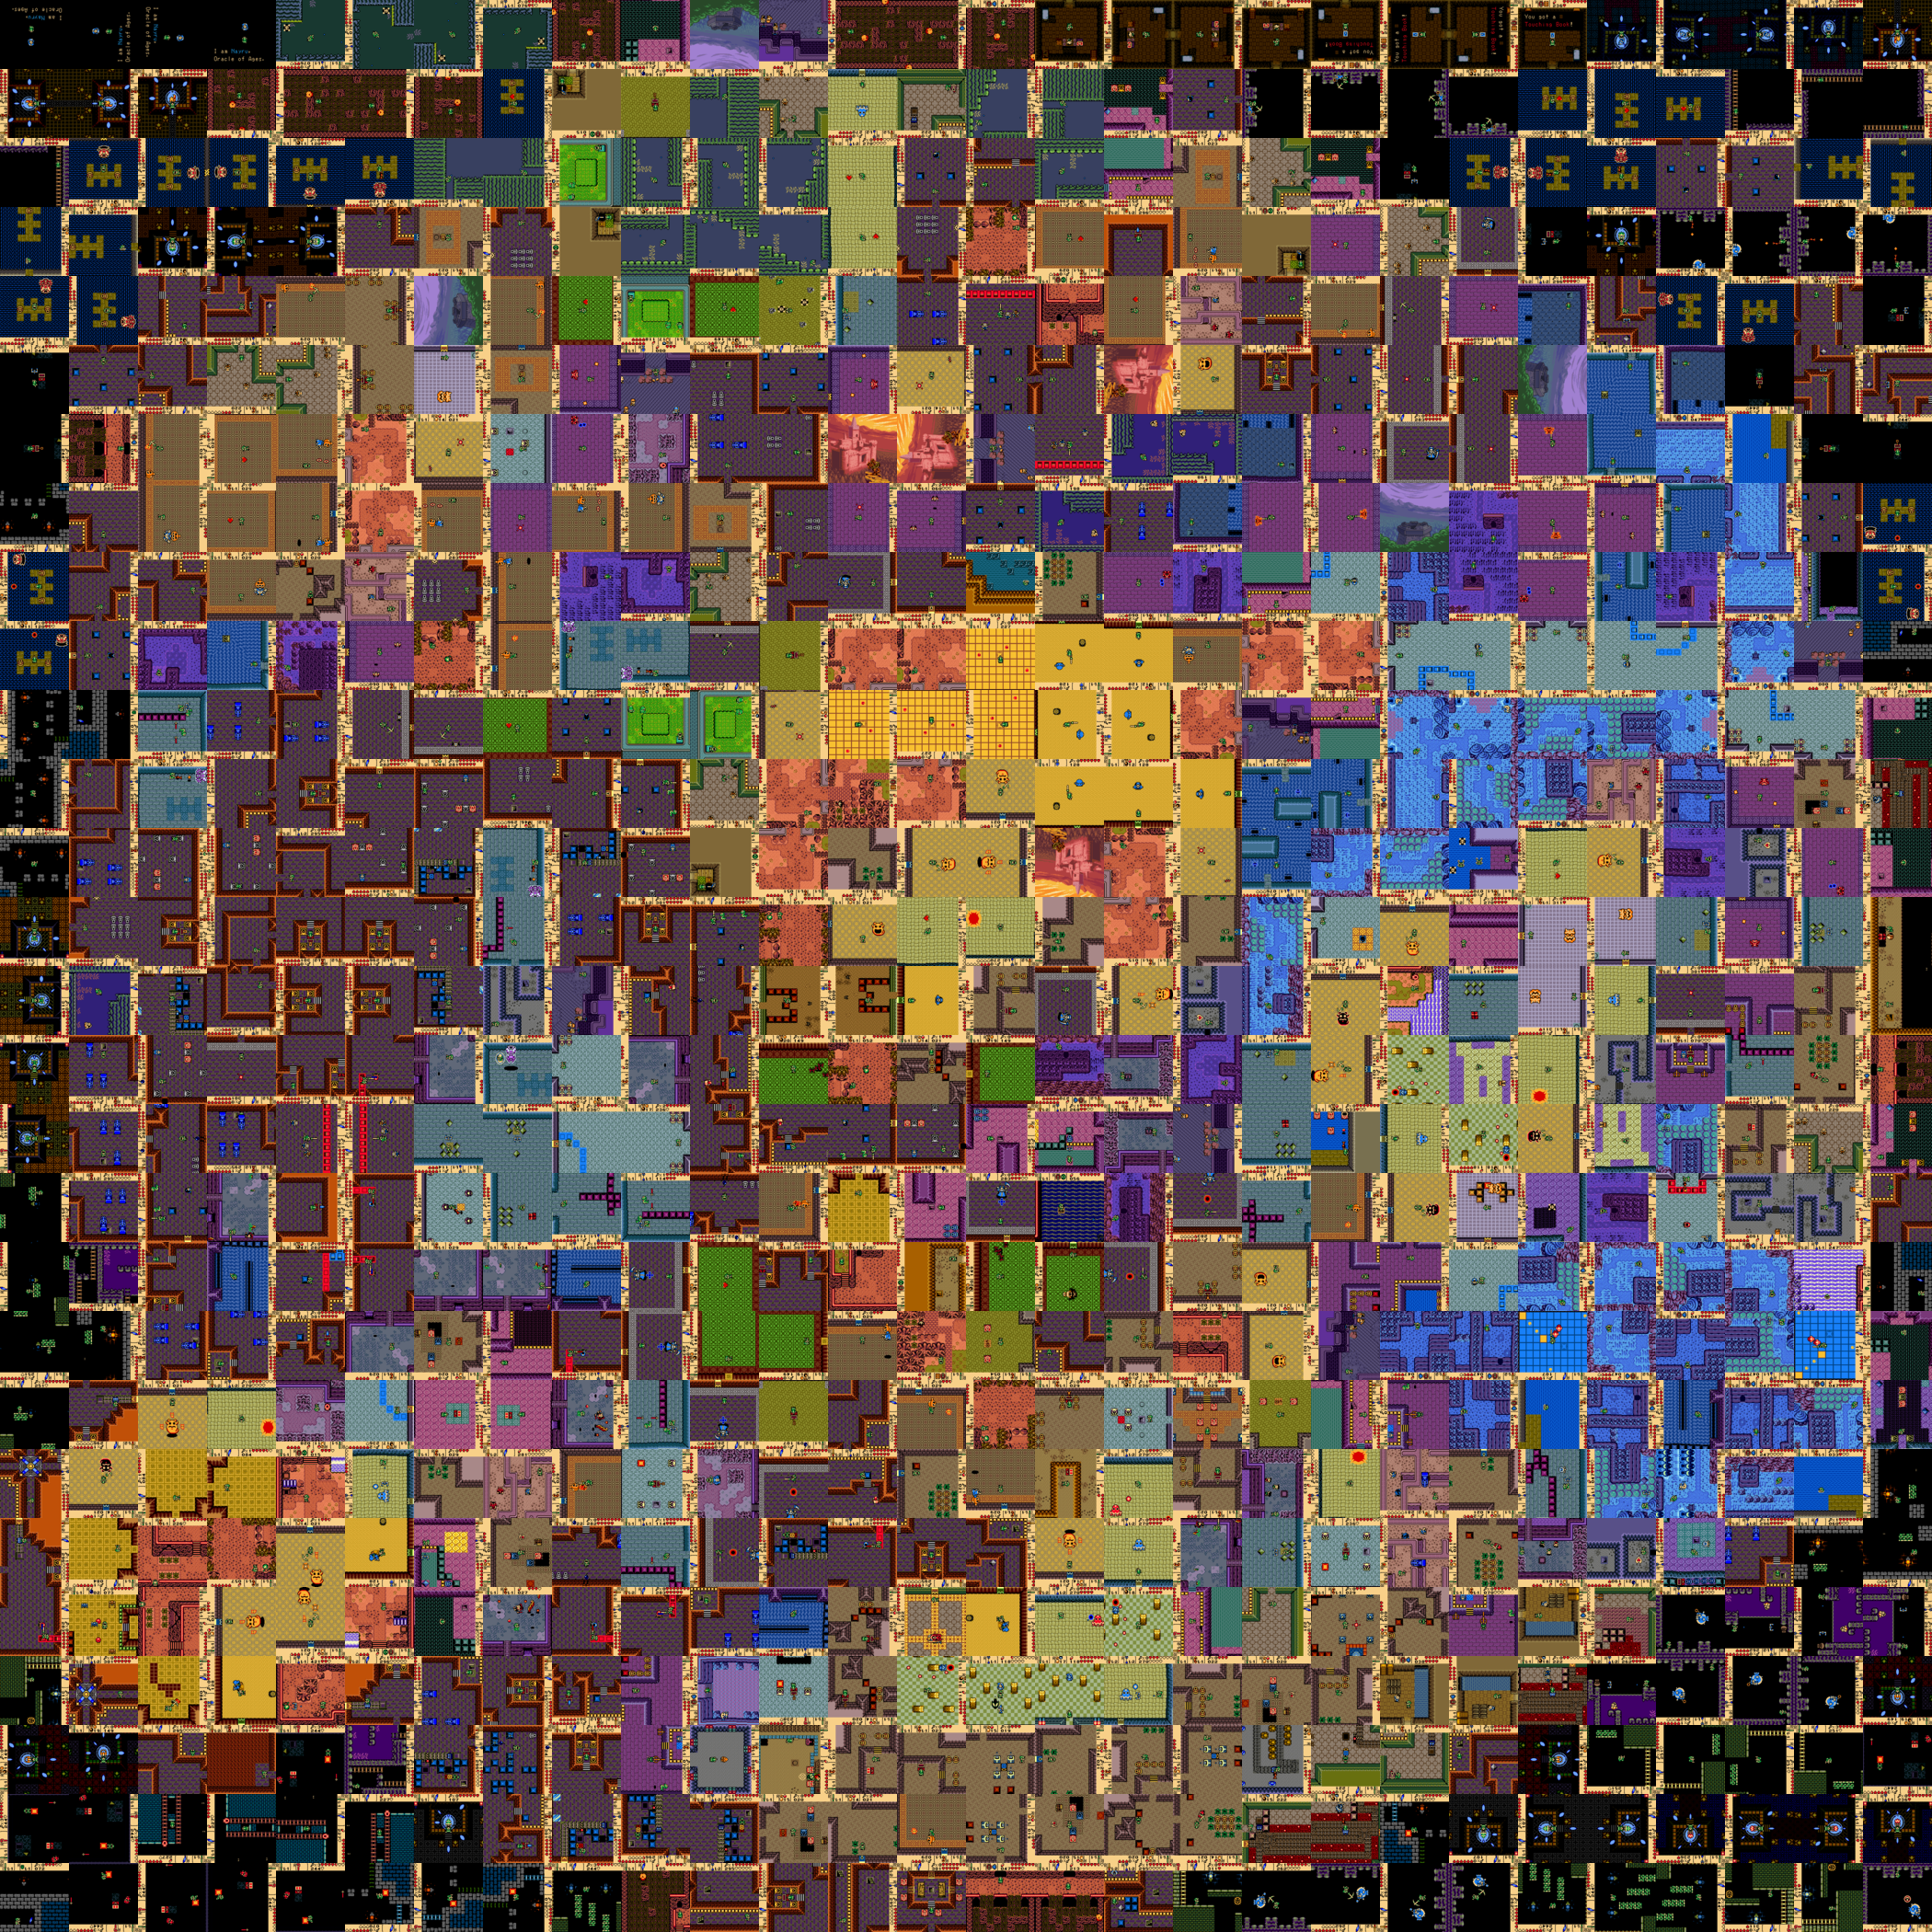
\includegraphics[width=\linewidth]{img/oracle_of_ages_v2.png}
        \caption{Version 2 Mosaic}
    \end{subfigure}
    \begin{subfigure}{0.35\textwidth}
        \includegraphics[width=\linewidth]{img/oracle_of_ages_v3.png}
        \caption{Version 3 Mosaic}
    \end{subfigure}
    \begin{subfigure}{0.35\textwidth}
        \includegraphics[width=\linewidth]{img/oracle_of_ages_v1_smaller.png}
        \caption{Version 1 Mosaic with smaller inputs}
    \end{subfigure}
    \begin{subfigure}{0.35\textwidth}
        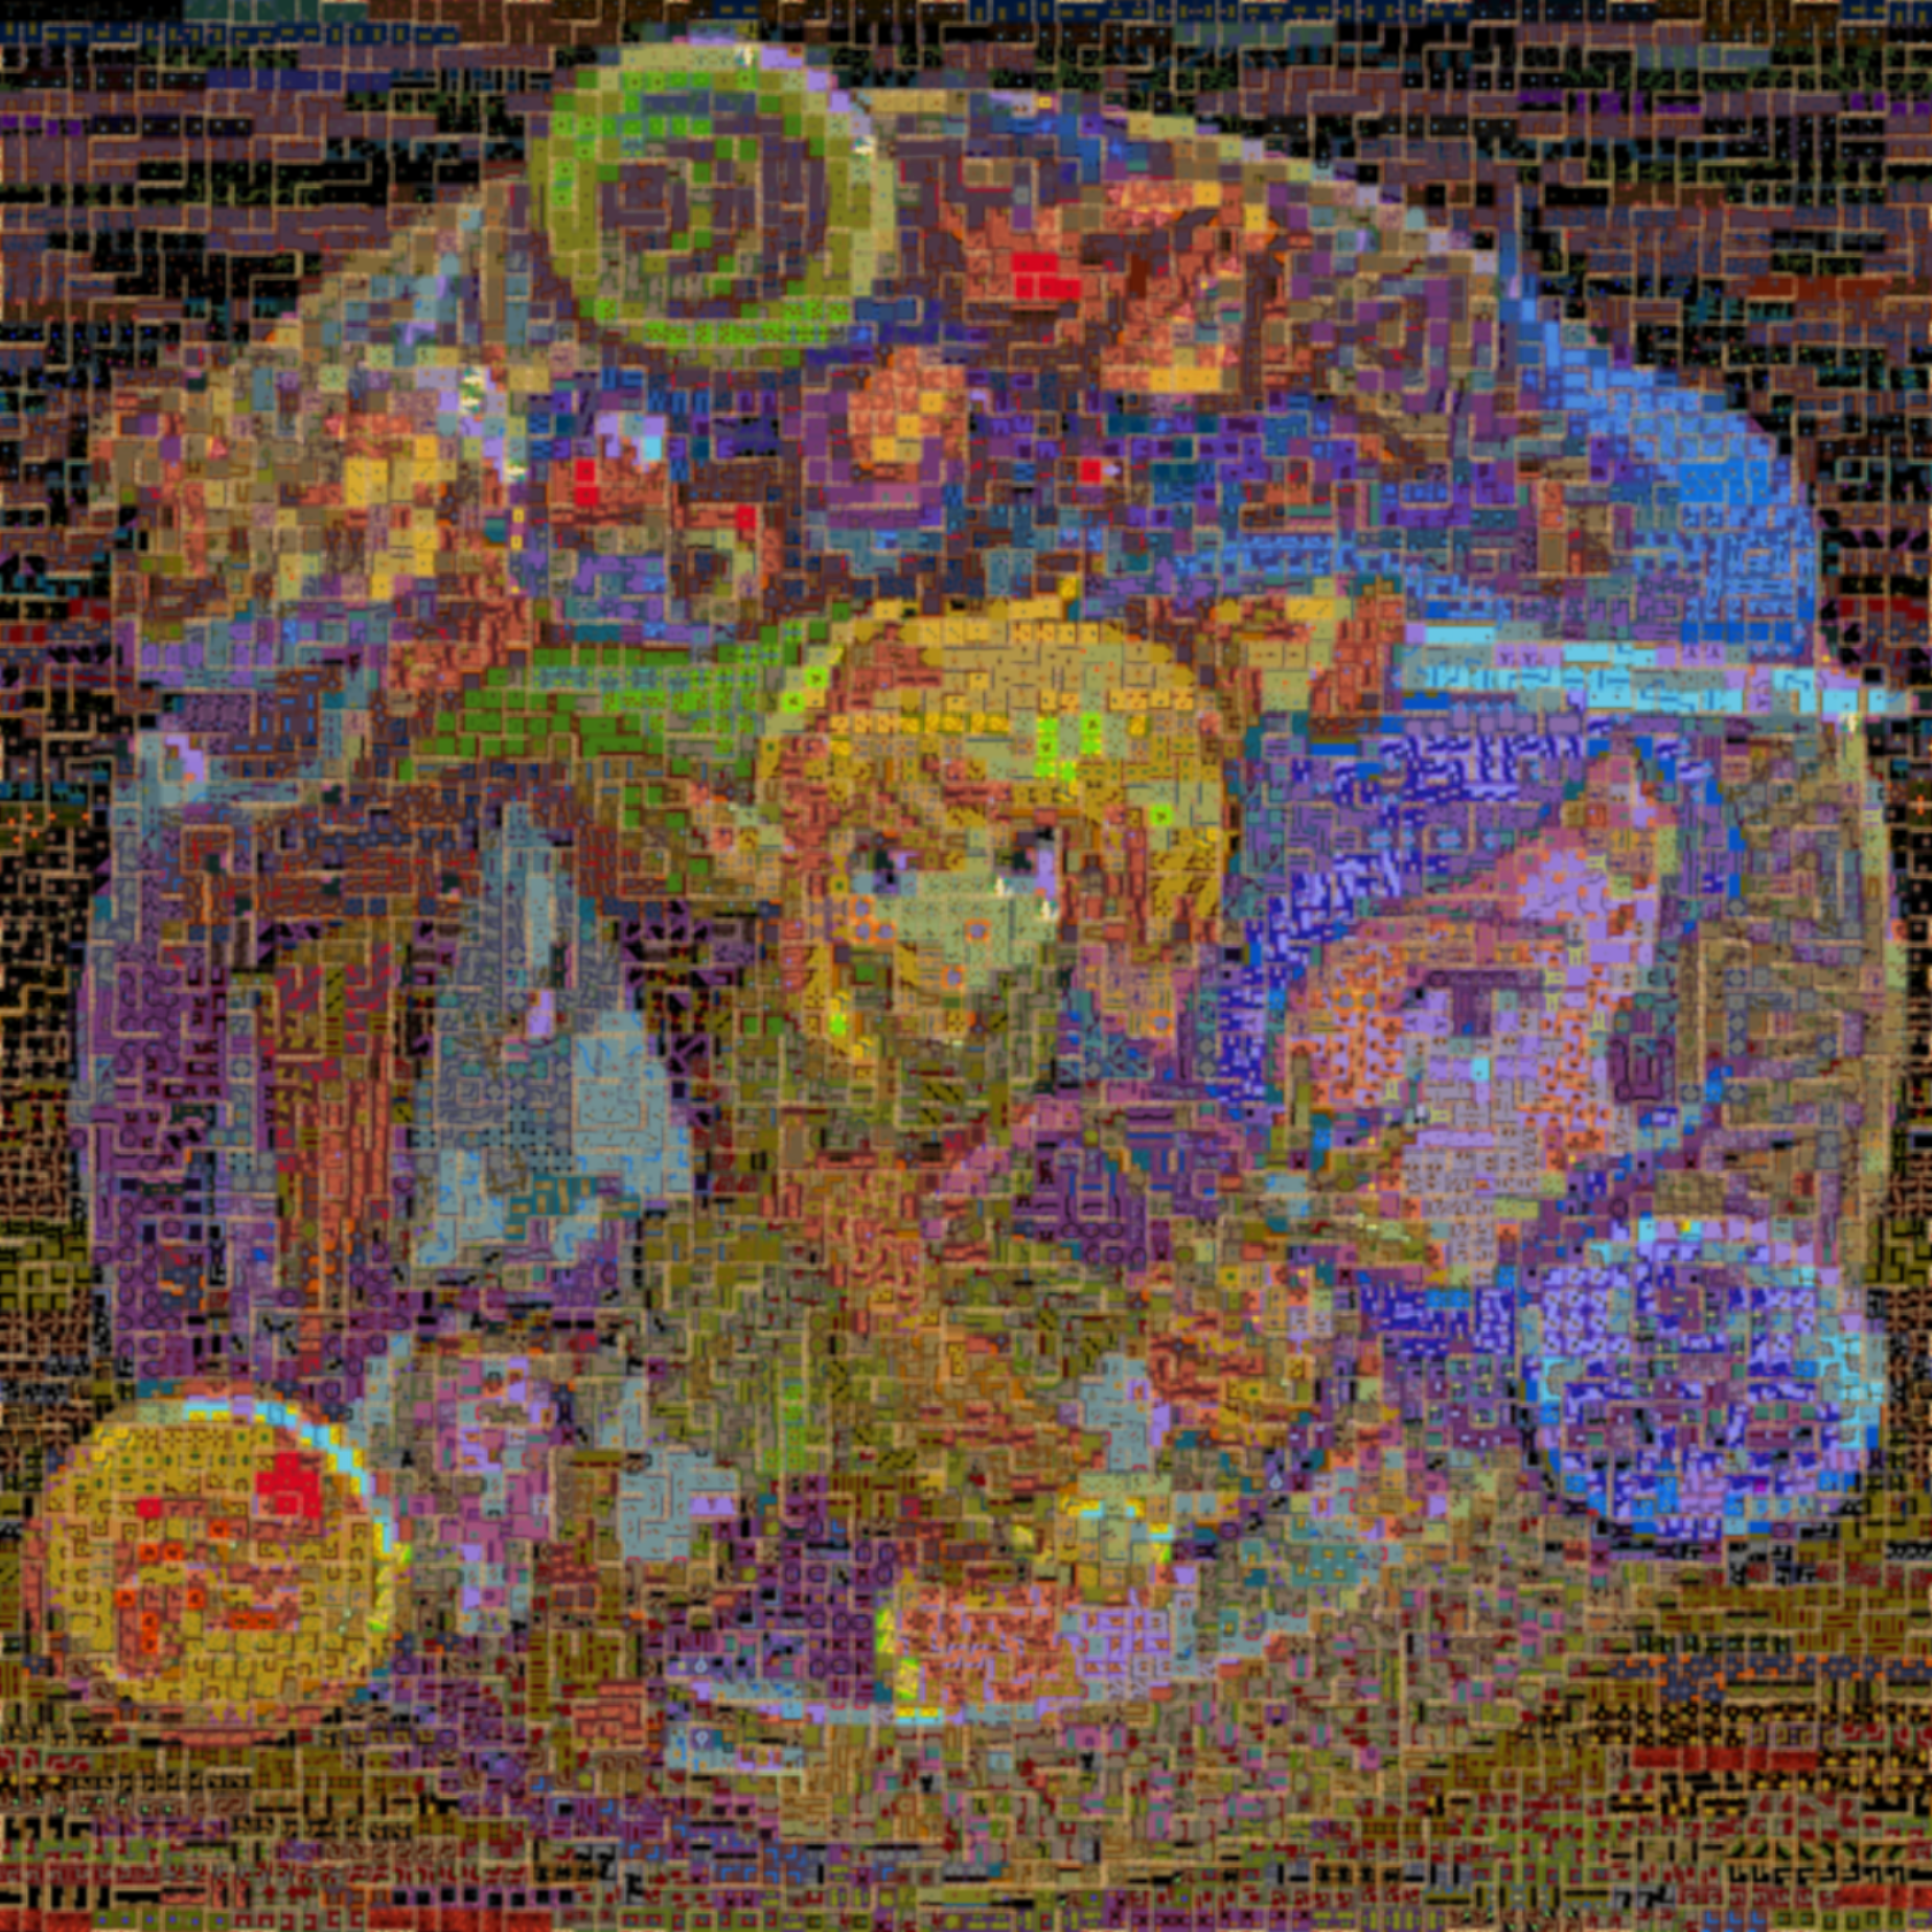
\includegraphics[width=\linewidth]{img/oracle_of_ages_v3_smaller.png}
        \caption{Version 3 Mosaic with smaller inputs}
    \end{subfigure}
    \caption{\texttt{zelda-mosaic} sample}\label{F:zelda-mosaic-sample}
\end{figure*}

We iteratively developed three versions after our initial proof-of-concept. Each
version refines the algorithm of the previous version (for details,
see~\ref{S:AlgDet}). Starting from a working prototype (version
1,~\ref{S:algv1}), we proceeded to add limited duplication (version
2,~\ref{S:algv2}) and seam-blending (version 3,~\ref{S:algv3}). We also further
refined mosaic quality by stitching smaller images, at a performance cost. The
original presentation is publicly available~\cite{zelda_mosaic_pres}, as is a
separate video-recording~\cite{zelda_mosaic_vid}.

Now we propose to examine these algorithms as implemented in the MATLAB source
and prove, if possible, their termination given well-conditioned input. What
necessary conditions are remains to be seen, but likely includes constraints on
the sizes of each individual input image and the size of the key art target
image.

\subsection{Motivation}

There are several factors that motivate our interest in this particular
algorithm, its particular implementation, and its properties.

Personally, it is a project we've already invested in, and one which we enjoy
studying.

Academically, it presents several unique opportunities. First, as far as we can
tell, there have been no studies on either termination-properties of mosaic
algorithms or of MATLAB code. Further, we have found no attempt to formalize
details of the MATLAB programming language\footnote{This may in part be due to
the proprietary, closed-source nature of MATLAB\@. Nevertheless, we hope to make
an attempt, though it must be grounded in the knowledge that any proof can only
hold if indeed the MATLAB environment faithfully implements the semantics it
claims. There are formalizations of a particular MATLAB toolkit known as
Stateflow~\cite{Hamon_2005,Hamon_2007} but none that we have found for general
MATLAB programming.}. Thus already in studying this particularly narrow problem
we have an opportunity to extend the space of studies in formal-methods and
their applications to the programmer and their programs.

Second, we as students of these formal methods lack experience in formalizing
these details about specific algorithms. The Logical Foundations
text~\cite{Pierce:SF1} has proven a great resource in learning about these
principles on small examples, and our study of \texttt{zelda-mosaic} will make
an excellent opportunity to extend our practical knowledge of the field.

Lastly, termination and its decidability has always been a study of interest to
the logician, the mathematician, and the computer scientist. From Hilbert's
\textit{Entscheidungsproblem} to Turing's Halting problem~\cite{Cook_2011}, the
world of algorithms is generally concerned with what is, indeed, computable.
While we make no attempt here to prove termination of arbitrary or even
restricted MATLAB programs (likely a Sisyphean task), we can at least attempt to
push the boundaries of the undecidable Halting problem for this specific
program.

\section{Algorithm Details}\label{S:AlgDet}

In this section, we present the high-level details of the three algorithms about
which we aim to prove termination. We begin with a brief overview of the
relevant inputs before proceeding to give pseudo MATLAB-code for each version of
the algorithm accompanied by textual explanation.

\subsection{Background}

Across each of the three versions, the inputs are the same. The three inputs are

\begin{enumerate}
    \item an image \textit{key art}, the target image the final mosaic will
        replicate
    \item a series of \textit{thumbnails}, smaller images which will form the
        tiles of the mosaic
    \item an integer \textit{size}, corresponding to the side-length of the
        square thumbnails
\end{enumerate}

In the larger versions, we used a size of 75 pixels. In the smaller versions, we
used 25 pixels. Each piece of key art is expected to have dimensions
integer-multiples of the size input.

The final output is a \textit{mosaic} of dimensions identical to the key art,
where every \(size \times size\)-pixel subset is an image selected from the
thumbnails.

The MATLAB program reads these images, manipulates them as a \textit{cell
array}\footnote{This is MATLAB's dynamically sized data-structure} of RGB
values, and the result was written into a PNG file. Aside from general MATLAB
control flow constructs, our code uses the built-in \textit{immse}~\cite{immse}
function to calculate pixel-level differences between two images and the
external \textit{MAT2TILES}~\cite{mat2tiles} library to break the key art images
into tiles in a cell array format.

\subsection{Algorithm for version 1}\label{S:algv1}

Our first version of the algorithm is straightforward. It divides the key art
into \(size \times size\)-pixel chunks. Each chunk is replaced with the
corresponding ``best'' thumbnail. Here, ``best'' means the thumbnail with the
lowest mean-squared error when compared to the original chunk. Details are
reproduced in \figurename~\ref{alg:v1}.

\begin{figure}[!t]
    \textbf{Input}: image \(key\_art\), images \(thumbnails\), integer \(size\) \\
    \textbf{Output}: image \(tiles\)
    \begin{algorithmic}
        \STATE{\(tiles \gets \textrm{MAT2TILES}(key\_art, size, size)\)}
        \FOR{\(tile \in tiles\)}
            \FOR{\(thumbnail, i \in thumbnails, [1..|thumbnails|]\)}
                \STATE{\(mses_i \gets \textrm{immse}(tile, thumbnail)\)}
            \ENDFOR
            \STATE{\(best\_indices \gets \textrm{find} (mses = \min mses)\)}
            \STATE{\(best\_index \gets best\_indices_0\)}
            \STATE{\(tile \gets thumbnails_{best\_index}\)}
        \ENDFOR
    \RETURN{\(tiles\)}
    \end{algorithmic}
    \caption{Algorithm: Version 1}\label{alg:v1}
\end{figure}

\subsection{Algorithm for version 2}\label{S:algv2}

The second version of the algorithm addresses a noticeable issue with our first
attempt---namely, there is nothing preventing the algorithm from reusing the
same thumbnail repeatedly, which can result in several recurrences of the same
image in the final mosaic. This produces a boring result, and many of our
version 1 outputs exhibit this repetition, in part because of the repeated use
of similar color throughout the key art.

This version of the algorithm keeps track of the thumbnails that have already
been used, up to a threshold. It will search for the ``next-best'' option if the
best thumbnails have already been used. Details are presented in
\figurename~\ref{alg:v2}.

The idea is to maintain a mapping from thumbnail to number of uses. When looking
for the best thumbnail for a given chunk, only a thumbnail that has not exceeded
the threshold in number of uses can be used. In effect, this limits each
thumbnail to a certain (typically small) number of uses, preventing gratuitous
repetition. This can also cause artifacts in the output, as we don't always get
the most representative thumbnail for a given chunk.

The threshold is chosen to allow thumbnails to be re-used enough to cover the
entire mosaic, but not more than is absolutely required.

\begin{figure}[!t]
    \textbf{Input}: image \(key\_art\), images \(thumbnails\), integer \(size\) \\
    \textbf{Output}: image \(tiles\)
    \begin{algorithmic}
        \STATE{\(tiles \gets \textrm{MAT2TILES}(key\_art, size, size)\)}
        \STATE{\(used \gets \emptyset\)}
        \STATE{\(threshold \gets 1\)}
        \IF{\(|thumbnails| < |tiles|\)}
            \STATE{\(threshold \gets \lceil{|tiles| / |thumbnails|}\rceil\)}
        \ENDIF
        \FOR{\(tile \in tiles\)}
            \FOR{\(thumbnail, i \in thumbnails, [1..|thumbnails|]\)}
                \STATE{\(mses_i \gets \textrm{immse}(tile, thumbnail)\)}
            \ENDFOR
            \STATE{\(best\_indices \gets \textrm{find} (mses = \min mses)\)}
            \STATE{\(best\_index \gets best\_indices_0\)}
            \WHILE{\(used_{best\_index} \ge threshold\)}
                \STATE{\(mses_{best\_index} \gets \infty\)}
                \STATE{\(best\_indices \gets \textrm{find} (mses = \min mses)\)}
                \STATE{\(best\_index \gets best\_indices_0\)}
            \ENDWHILE
            \STATE{increment \(used_{best\_index}\)}
            \STATE{\(tile \gets thumbnails_{best\_index}\)}
        \ENDFOR
        \RETURN{\(tiles\)}
    \end{algorithmic}
    \caption{Algorithm: Version 2}\label{alg:v2}
\end{figure}

\subsection{Algorithm for version 3}\label{S:algv3}

The last noticeable issue we decided to tackle for version 3 was the seams
between individual chunks. They aren't as noticeable in the outputs with smaller
thumbnails, but in our original (\(75 \times 75\)) outputs there are visible
grid lines where the chunks meet.

To combat this, we tested a variety of blurring techniques to reduce the visual
impact of the seams. In the process, we also aimed for producing a more coherent
whole---i.e., a mosaic that looks more like a true image than a tiled grid.

We settled on combination of two techniques. The first technique is to blur the
entire mosaic with a Gaussian filter (via the \textit{imgaussfilt} function),
smoothing the image. The second technique is to blur each of the horizontal and
vertical seams by replacing a narrow band around the seam with the average of
the pixels in that region. Pseudocode is presented in \figurename~\ref{alg:v3}.

\begin{figure}[!t]
    \textbf{Input}: image \(key\_art\), images \(thumbnails\), integer \(size\) \\
    \textbf{Output}: image \(tiles\)
    \begin{algorithmic}
        \STATE{}\COMMENT{Repeat Version 2}
        \STATE{\(tiles \gets \textrm{Version2}(key\_art, thumbnails, size)\)}
        \STATE{\(tiles \gets \textrm{imgaussfilt}(tiles)\)}
        \STATE{\(strip\_size \gets \lfloor{size / 8}\rfloor\)}
        \STATE{}\COMMENT{Blur by averaging}
        \FOR{horizontal \(strip \in tiles\)}
            \STATE{\(strip \gets \textrm{mean}({strip})\)}
        \ENDFOR
        \FOR{vertical \(strip \in tiles\)}
            \STATE{\(strip \gets \textrm{mean}({strip})\)}
        \ENDFOR
        \RETURN{\(tiles\)}
    \end{algorithmic}
    \caption{Algorithm: Version 3}\label{alg:v3}
\end{figure}

\section{Related Work}

Because we are proving something about code that we have written ourselves,
there is not a vast body of literature specific to our algorithms from which we
can draw. There are however a number of related issues exposed by our code,
which we will discuss here. In particular, the following are of interest and
have been written about:

\begin{itemize}
    \item The correctness of MATLAB's \textit{cell array} data structure and its
        representation in Coq;
    \item The correctness of MATLAB's built-in numerical functions and matrix
        operations; and
    \item Proving termination of a particular program based on the inputs of the
        program.
\end{itemize}

Since our program deals with a large amount of pixel information in memory as a
matrix, it may be instructive to ensure that the representation of our data is
robust and that assumptions made about them lead to the results that we expect.
We are not the first group to demonstrate interest in proving properties about
matrix representations. In the early days of Coq, a
paper~\cite{magaud:hal-00955444} was published discussing the implementation of
square matrices in Coq, as well as proofs involving basic operations such as
addition and multiplication. This paper references \textit{Linear
Algebra}~\cite{lin_alg}, a Coq library written by a colleague which formalizes
a well-known linear algebra text~\cite{linear_algebra} and supports matrices with
a differing number of rows and columns. It is not known at this time how these
implementations compare with built-in Coq modules, but it will be useful to
reference external matrix proofs and see how we might make similar arguments
about matrix representations as they apply to our code.

MATLAB is a closed-source piece of software, and little has been published about
its correctness. In the official MATLAB forum, users have demonstrated interest
in verifying the correctness of MATLAB algorithms~\cite{duenisch_2013} and the
MATLAB staff reassure users that the algorithms have gone through rigorous
testing, but this assurance does not carry the same weight as a formal
verification. Indeed, as we have learned, these techniques fall on separate
parts of a correctness spectrum, with testing demonstrating correctness less
reliably than formal methods. The lack of related work in the MATLAB domain
serves as further motivation to obtain results about the correctness of a subset
of MATLAB features used in our code.

Program termination is a topic of wide interest in the computing community, as
it has both practical and of theoretical relevance given the famous halting
problem. \citeauthor{Cook_2011}~\cite{Cook_2011} argue in their article that
computer scientists are often hesitant to make claims about the termination of a
particular program, but that it is often achievable. Their work draws from the
field of compilers and makes the argument that one can prove the termination of
a program given certain inputs, provided that there is sufficient analysis of
the relation between the inputs and the possible paths that may be taken during
execution\footnote{In many contexts, this involves things like symbolic
execution (cf. Rosette~\cite{Rosette}).}. Many of the ideas in this work are
formalized by \citeauthor{BLANQUI_2011} in the \textit{CoLoR} library for Coq,
which is used primarily for proofs involving rewriting code and program
termination~\cite{BLANQUI_2011}. These efforts demonstrate that the field is
rich with material that relates termination and inputs, and, while we likely
won't make significant contributions to this work, it will be interesting to see
how well these arguments translate to the domain of scientific computing.

\section{Timeline}

Given the exploratory nature of this project, we may need to modify the
properties we decide to prove and the scope of the project as we learn more
about implementing our structures in Coq and decide the extent to which we can
model elements of MATLAB code. Taking this into consideration, we estimate the
following to be to be a reasonable timeline of project completion:

\begin{itemize}
    \item \textbf{03/01/21}: Project Proposal Due
    \item \textbf{03/15/21}: Represent relevant data structures in Coq, as well
        as primitive operations for matrix manipulation and accesses.
    \item \textbf{03/29/21}: Scope of project finalized with formal problem
        specification; sketch of theorems and lemmas that we expect to write in
        the process of writing our proof.
    \item \textbf{03/31/21}: Progress Report Due
    \item \textbf{04/09/21}: Significant progress made on most theorems and
        lemmas.
    \item \textbf{04/19/21}: Most theorems and lemmas should be complete; change
        scope of project where necessary.
    \item \textbf{04/24/21}: All logic should be implemented; edits for readability should be the only changes henceforth.
    \item \textbf{04/26/21}: Final Proof Due
    \item \textbf{05/03/21}: Final Paper Due
    \item \textbf{05/05/21}: Final Presentation Delivered
\end{itemize}

\section{Contribution Report}

D. B. Knoble contributed the abstract, introduction, and motivation. He also
contributed to the explanations of the algorithms. J. Do contributed the
majority of the algorithm details, as well as the related work and timeline.

{\printbibliography}

\end{document}
